\chapter{Sperimentazione del Protocollo}
\label{chap:sperimentazione}

Il collaudo finale del protocollo è stato condotto con due nodi basati su ESP32-WROOM-32, uno equipaggiato con 
l'altoparlante pilotato dal MAX98357A e l'altro con il microfono MEMS SPH0645LM4H descritti in \autoref{chap:implementazione_hardware}; 
i dispositivi sono stati alimentati da un'unica linea regolata e poggiati distanziati di 20cm per evitare 
riflessioni ravvicinate, mentre il firmware in \autoref{chap:implementazione_software} è
 stato compilato con gli stessi parametri su entrambe le schede.\\
  Nell'arco di una settimana sono stati effettuati tre blocchi di prove serali ognuna da circa 2 ore, 
 rispettivamente da 180, 220 e 160 trasmissioni consecutive, per un totale di 560 pacchetti analizzati: ogni campagna prevedeva l'avvio automatico 
 della sequenza di configurazione, la pubblicazione del comando "movement\_sensor\_on" oppure "movement\_sensor\_on\_" susseguito da un tempo casuale in miillisecondi; 
 ogni richiesta quindi prevedeva l'impiego durante la fase di configurazione ma anche durante l'emissione del comando, l'utilizzo di un ID sequenziale, 
 quindi diverso ad ogni invio, nel range tra 0000 e 0560, e infine
 l'invio di un messaggio telemetrico che riproduceva un timestamp decimale.\\
  Per ogni scambio il timer integrato nel processore dell'ESP32 ha registrato la finestra di trasmissione e i log generati
  da \textbf{estimate\_send\_duration}, successivamente in automatico uno \textbf{script Python} ha ricalcolato convertendo le stringhe ASCII
   in caratteri a sette bit e comprimendole con la tabella run-length di \autoref{tab:freq_codici}, verificando che il calcolo corrispondesse.\\
   Inoltre il software di ricezione ha salvato anche il conteggio delle ritrasmissioni a seguito di una trasmissione non confermata.

\definecolor{lightgray}{RGB}{235,235,235}
\definecolor{white}{RGB}{255,255,255}

\begin{table}[H]
    \centering
    \resizebox{\textwidth}{!}{%       
    \begin{tabular}{|>{\raggedright\arraybackslash}p{3.3cm}|>{\columncolor{lightgray}}c|>{\columncolor{lightgray}}c|>{\columncolor{lightgray}}c|>{\columncolor{lightgray}}c|>{\columncolor{lightgray}}c|}
        \hline
        \textbf{Scenario} & \textbf{Prove} & \textbf{Signal code medi} & \textbf{Tempo medio [ms]} & \textbf{Bitrate utile [bps]} & \textbf{Ritrasmissioni [\%]} \\
        \hline
        Configurazione (REQ/SET/OK) & 180 & 171 & 26232 & 14.7 & 0.9 \\
        Movement sensor ON & 220 & 239 & 36568 & 14.0 & 0.6 \\
        Telemetria ASCII ``1738450195'' & 160 & 155 & 23720 & 14.5 & 0.8 \\
        \hline
    \end{tabular}
    }

    \caption{Sintesi numerica delle tre campagne sperimentali condotte sul protocollo audio}
    \label{tab:risultati_sperimentali}
\end{table}

I dati aggregati in \autoref{tab:risultati_sperimentali} mostrano che la registrazione\\
 (sequenza \textbf{REQ/SET/OK} del Livello Link descritta in \autoref{sec:livello_link}) produce in media 
 171 signal code per scambio, pari a \SI{385}{bit} utili trasmessi in \SI{26.232}{\second} con un bitrate che
  si attesta sui \SI{14.7}{\bit\per\second}. \\ 
  Il comando "movement\_sensor\_on" codificato come\\ \textbf{ID:0471\{MOVEMENT\_ON\}k\{0000\}} 
  e la successiva risposta  \\
  \textbf{ID:0000\{MOVEMENT\_YES\}k\{0471\}} totalizzano 239 signal code, equivalenti a \SI{36.568}{\second} di
   trasmissione e a un'efficienza di \SI{14.0}{\bit\per\second}; la variante con parametro temporale \textbf{MOVEMENT\_ON\_12000} ha generato 
   in laboratorio 107 signal code solo per il comando, confermando quanto l'assenza di coppie ripetute nelle cifre ASCII penalizzi la compressione
    run-length descritta in \autoref{chap:implementazione_software}.\\
     Anche la trama telemetrica "1738450195", inviata con il prefisso\\
     \textbf{ID:0471\{DATA\}k\{0000\}}, si ferma a \SI{14.5}{\bit\per\second} perché la distribuzione semi-alternata dei bit obbliga il \autoref{sec:livello_link}
      a cambiare segno quasi ogni due posizioni, \textbf{riducendo l'ampiezza media dei run a poco più di due bit}.\\
        La media complessiva del bitrate utile su tutte le prove si attesta a \SI{14.4}{\bit\per\second}, in linea con quanto affermato nella \autoref{sec:livello_bit}.\\

\begin{figure}[H]
    \centering
    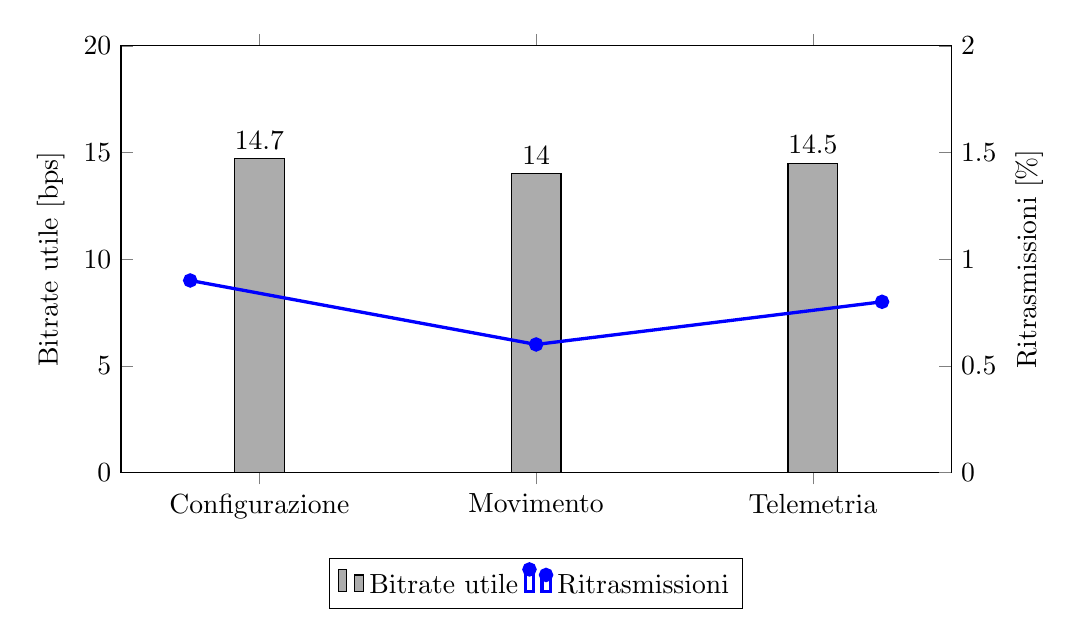
\begin{tikzpicture}
        \begin{axis}[
            width=\textwidth,
            height=7cm,
            ybar,
            bar width=18pt,
            ymin=0,
            ymax=20,
            enlarge x limits=0.25,
            ylabel={Bitrate utile [bps]},
            symbolic x coords={Configurazione, Movimento, Telemetria},
            xtick=data,
            legend style={at={(0.5,-0.2)}, anchor=north, legend columns=2},
            legend cell align=left,
            nodes near coords,
            nodes near coords align={vertical}
        ]
            \addplot[fill=gray!65] coordinates {(Configurazione,14.7) (Movimento,14.0) (Telemetria,14.5)};
            \addlegendentry{Bitrate utile}
            \addlegendimage{color=blue, mark=*, very thick}
            \addlegendentry{Ritrasmissioni}
        \end{axis}
        \begin{axis}[
            width=\textwidth,
            height=7cm,
            axis y line*=right,
            axis x line=none,
            ymin=0,
            ymax=2,
            ylabel={Ritrasmissioni [\%]},
            symbolic x coords={Configurazione, Movimento, Telemetria},
            xtick=data
        ]
            \addplot[color=blue, mark=*, very thick] coordinates {(Configurazione,0.9) (Movimento,0.6) (Telemetria,0.8)};
        \end{axis}
    \end{tikzpicture}
    \caption{Trend del bitrate utile e della percentuale di ritrasmissioni misurati nelle tre casistiche di prova}
    \label{fig:trend_bitrate}
\end{figure}

La bassa percentuale di ritrasmissioni riportata nel grafico deriva da un meccanismo di conferma
 continua che obbliga il nodo ricevente a replicare \textbf{l'acknowledgement} sul canale slave o master entro \SI{100}{\milli\second} dalla decodifica del frame;
  lo schema temporale di \autoref{fig:timeline_pacchetto} 
  mostra come l'unico NACK (nessun ACK) registrato durante la sequenza di configurazione venga seguito dal reinvio di un singolo pacchetto e \\
  dalla successiva conferma positiva, penalizzando il tempo complessivo della macro-operazione.\\
   Anche nei cicli telemetrici più gravosi la logica di ritrasmissione non ha richiesto più di un tentativo aggiuntivo e,
    grazie alla persistenza di fase nel generatore audio di \autoref{chap:implementazione_software}, 
    l'aggancio dello spettro è rimasto stabile.

\begin{figure}[H]
    \centering
    \begin{tikzpicture}[>=Latex, line width=1pt]
        \draw[thick] (-0.5,1.4) -- (9.5,1.4);
        \draw[thick] (-0.5,0) -- (9.5,0);
        \node[above left] at (-0.5,1.4) {Trasmettitore};
        \node[below left] at (-0.5,0) {Ricevitore};

        \draw[->] (0,1.4) -- (1.2,0) node[midway, left] {1: Req};
        \draw[->] (1.4,0) -- (2.6,1.4) node[midway, left] {2: Set};
        \draw[->, dashed] (2.8,1.4) -- (4,0) node[midway, left] {NACK};

        \draw[->] (4.2,0) -- (5.4,1.4) node[midway, left] {2: Set};
        \draw[->] (5.6,1.4) -- (6.8,0) node[midway, right] {ACK};
    \end{tikzpicture}
    \caption{Sequenza temporale semplificata con l'unica ritrasmissione registrata durante la fase di configurazione}
    \label{fig:timeline_pacchetto}
\end{figure}